%%=============================================================================
%% LaTeX sjabloon voor bachelorproef, HoGent Bedrijf en Organisatie
%% Opleiding Toegepaste Informatica
%%=============================================================================

\documentclass[fleqn,a4paper,12pt]{book}

%%=============================================================================
%% LaTeX sjabloon voor de bachelorproef, HoGent Bedrijf en Organisatie
%% Opleiding toegepaste informatica
%%
%% Structuur en algemene vormgeving. Meestal hoef je hier niets te wijzigen.
%%
%% Vormgeving gebaseerd op "The Legrand Orange Book", version 2.0 (9/2/15)
%% door Mathias Legrand (legrand.mathias@gmail.com) met aanpassingen door
%% Vel (vel@latextemplates.com). Het oorspronkelijke template is te vinden op
%% http://www.LaTeXTemplates.com
%%
%% Aanpassingen voor HoGent toegepaste informatica: 
%%   Bert Van Vreckem <bert.vanvreckem@hogent.be>
%% Licentie: 
%%   CC BY-NC-SA 3.0 (http://creativecommons.org/licenses/by-nc-sa/3.0/)
%%=============================================================================

%%-----------------------------------------------------------------------------
%% Packages
%%-----------------------------------------------------------------------------

\usepackage[top=3cm,bottom=3cm,left=3cm,right=3cm,headsep=10pt,a4paper]{geometry} % Page margins
\usepackage[utf8]{inputenc}  % Accenten gebruiken in tekst (vb. é ipv \'e)
\usepackage{amsfonts}        % AMS math packages: extra wiskundige
\usepackage{amsmath}         %   symbolen (o.a. getallen-
\usepackage{amssymb}         %   verzamelingen N, R, Z, Q, etc.)
\usepackage[english,dutch]{babel}    % Taalinstellingen: woordsplitsingen,
                             %  commando's voor speciale karakters
                             %  ("dutch" voor NL)
\usepackage{iflang}
\usepackage{eurosym}         % Euro-symbool €
\usepackage{geometry}
\usepackage{graphicx}        % Invoegen van tekeningen
\graphicspath{{img/}}       % Specifies the directory where pictures are stored
\usepackage{tikz}            % Required for drawing custom shapes
\usepackage[pdftex,bookmarks=true]{hyperref}
                             % PDF krijgt klikbare links & verwijzingen,
                             %  inhoudstafel
\usepackage{enumitem}        % Customize lists
\setlist{nolistsep}         % Reduce spacing between list items
\usepackage{listings}        % Broncode mooi opmaken
\usepackage{multirow}        % Tekst over verschillende cellen in tabellen
\usepackage{rotating}        % Tabellen en figuren roteren

\usepackage{booktabs}        % Required for nicer horizontal rules in tables

\usepackage{xcolor}          % Required for specifying colors by name
\definecolor{maincolor}{RGB}{0,147,208} % Define the main color used for 
                             % highlighting throughout the book
                             % 0, 147, 208 = officiële kleur HoGent FBO

% Paragraph style: no indent, add space between paragraphs
\setlength{\parindent}{0em}
\setlength{\parskip}{1em}

\usepackage{etoolbox}
\usepackage{titling} % Macros for title, author, etc
\usepackage{lipsum}          % Voor vultekst (lorem ipsum)

%----------------------------------------------------------------------------------------
%	FONTS
%----------------------------------------------------------------------------------------

\usepackage{avant} % Use the Avantgarde font for headings
%\usepackage{times} % Use the Times font for headings
\usepackage{mathptmx} % Use the Adobe Times Roman as the default text font together with math symbols from the Sym­bol, Chancery and Com­puter Modern fonts

\usepackage{microtype} % Slightly tweak font spacing for aesthetics
\usepackage[utf8]{inputenc} % Required for including letters with accents
\usepackage[T1]{fontenc} % Use 8-bit encoding that has 256 glyphs

%------------------------------------------------------------------------------
%	TITLE PAGE
%------------------------------------------------------------------------------

\newcommand{\inserttitlepage}{%
\begin{titlepage}
  \newgeometry{top=2cm,bottom=1.5cm,left=1.5cm,right=1.5cm}
  \begin{center}

    \begingroup
    \rmfamily
    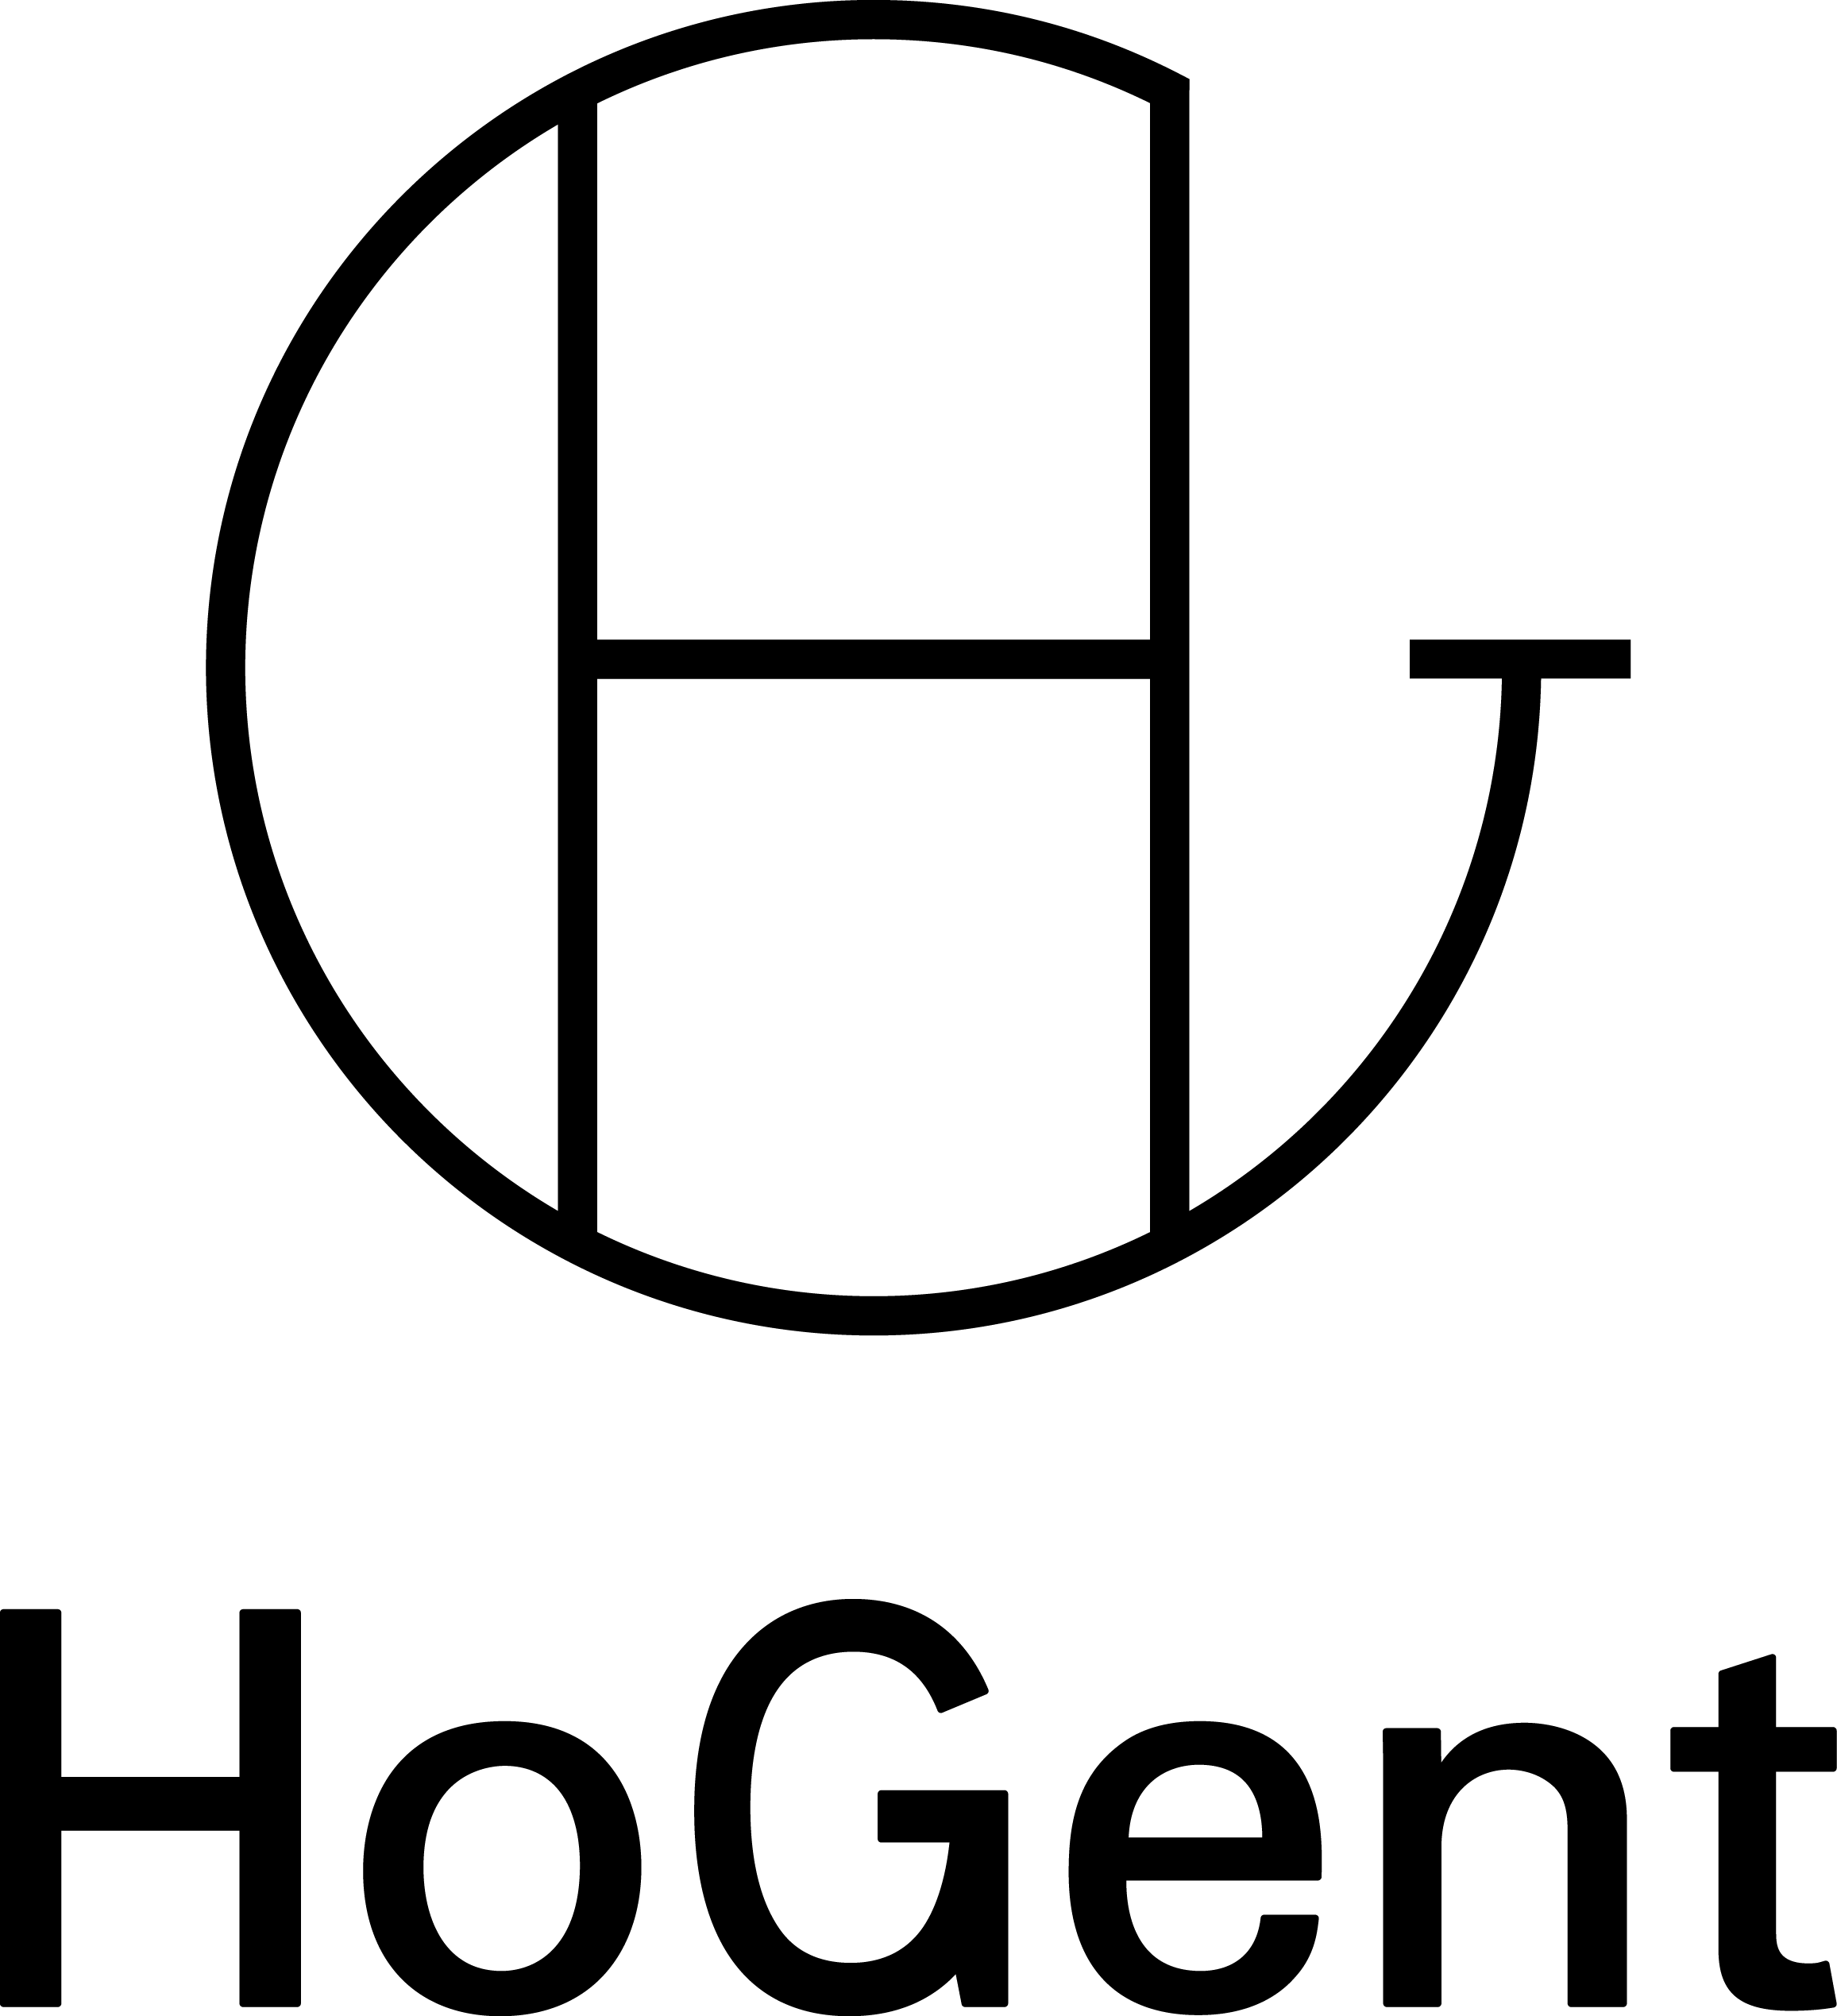
\includegraphics[width=2.5cm]{img/HG-beeldmerk-woordmerk}\\[.5cm]
    Faculteit Bedrijf en Organisatie\\[3cm]
    \titel
    \vfill
    \student\\[3.5cm]
    Scriptie voorgedragen tot het bekomen van de graad van\\professionele bachelor in de toegepaste informatica\\[2cm]
    Promotor:\\
    \promotor\\
    \ifdefempty{\copromotor}{\vspace{2.5cm}}{Co-promotor:\\\copromotor\\[2.5cm]}
    Instelling: \instelling\\[.5cm]
    Academiejaar: \academiejaar\\[.5cm]
    \ifcase \examenperiode \or Eerste \or Tweede \else Derde \fi examenperiode
    \endgroup

  \end{center}
  \restoregeometry
\end{titlepage}
  \emptypage
\begin{titlepage}
  \newgeometry{top=5.35cm,bottom=1.5cm,left=1.5cm,right=1.5cm}
  \begin{center}

    \begingroup
    \rmfamily
    \IfLanguageName{dutch}{Faculteit Bedrijf en Organisatie}{Faculty of Business and Information Management}\\[3cm]
    \titel
    \vfill
    \student\\[3.5cm]
    \IfLanguageName{dutch}{Scriptie voorgedragen tot het bekomen van de graad van\\professionele bachelor in de toegepaste informatica}{Thesis submitted in partial fulfilment of the requirements for the degree of\\professional bachelor of applied computer science}\\[2cm]
    Promotor:\\
    \promotor\\
    \ifdefempty{\copromotor}{\vspace{2.5cm}}{Co-promotor:\\\copromotor\\[2.5cm]}
    \IfLanguageName{dutch}{Instelling}{Institution}: \instelling\\[.5cm]
    \IfLanguageName{dutch}{Academiejaar}{Academic year}: \academiejaar\\[.5cm]
    \IfLanguageName{dutch}{%
    \ifcase \examenperiode \or Eerste \or Tweede \else Derde \fi examenperiode}{%
    \ifcase \examenperiode \or First \or Second \else Third \fi examination period}
    \endgroup

  \end{center}
  \restoregeometry
\end{titlepage}
}

%----------------------------------------------------------------------------------------
%	BIBLIOGRAPHY AND INDEX
%----------------------------------------------------------------------------------------

\usepackage[style=apa,backend=biber]{biblatex}
\usepackage{csquotes}
\DeclareLanguageMapping{dutch}{dutch-apa}
\addbibresource{bachproef-tin.bib} % BibTeX bibliography file
\addbibresource{../voorstel/voorstel.bib}
\defbibheading{bibempty}{}

\usepackage{calc} % For simpler calculation - used for spacing the index letter headings correctly
\usepackage{makeidx} % Required to make an index
\makeindex % Tells LaTeX to create the files required for indexing

%----------------------------------------------------------------------------------------
%	MAIN TABLE OF CONTENTS
%----------------------------------------------------------------------------------------

\usepackage{titletoc} % Required for manipulating the table of contents

\contentsmargin{0cm} % Removes the default margin

% Part text styling
\titlecontents{part}[0cm]
{\addvspace{20pt}\centering\large\bfseries}
{}
{}
{}

% Chapter text styling
\titlecontents{chapter}[1.25cm] % Indentation
{\addvspace{12pt}\large\sffamily\bfseries} % Spacing and font options for chapters
{\color{maincolor!60}\contentslabel[\Large\thecontentslabel]{1.25cm}\color{maincolor}} % Chapter number
{\color{maincolor}}
{\color{maincolor!60}\normalsize\;\titlerule*[.5pc]{.}\;\thecontentspage} % Page number

% Section text styling
\titlecontents{section}[1.25cm] % Indentation
{\addvspace{3pt}\sffamily\bfseries} % Spacing and font options for sections
{\contentslabel[\thecontentslabel]{1.25cm}} % Section number
{}
{\hfill\color{black}\thecontentspage} % Page number
[]

% Subsection text styling
\titlecontents{subsection}[1.25cm] % Indentation
{\addvspace{1pt}\sffamily\small} % Spacing and font options for subsections
{\contentslabel[\thecontentslabel]{1.25cm}} % Subsection number
{}
{\ \titlerule*[.5pc]{.}\;\thecontentspage} % Page number
[]

% List of figures
\titlecontents{figure}[0em]
{\addvspace{-5pt}\sffamily}
{\thecontentslabel\hspace*{1em}}
{}
{\ \titlerule*[.5pc]{.}\;\thecontentspage}
[]

% List of tables
\titlecontents{table}[0em]
{\addvspace{-5pt}\sffamily}
{\thecontentslabel\hspace*{1em}}
{}
{\ \titlerule*[.5pc]{.}\;\thecontentspage}
[]

%----------------------------------------------------------------------------------------
%	MINI TABLE OF CONTENTS IN PART HEADS
%----------------------------------------------------------------------------------------

% Chapter text styling
\titlecontents{lchapter}[0em] % Indenting
{\addvspace{15pt}\large\sffamily\bfseries} % Spacing and font options for chapters
{\color{maincolor}\contentslabel[\Large\thecontentslabel]{1.25cm}\color{maincolor}} % Chapter number
{}
{\color{maincolor}\normalsize\sffamily\bfseries\;\titlerule*[.5pc]{.}\;\thecontentspage} % Page number

% Section text styling
\titlecontents{lsection}[0em] % Indenting
{\sffamily\small} % Spacing and font options for sections
{\contentslabel[\thecontentslabel]{1.25cm}} % Section number
{}
{}

% Subsection text styling
\titlecontents{lsubsection}[.5em] % Indentation
{\normalfont\footnotesize\sffamily} % Font settings
{}
{}
{}

%----------------------------------------------------------------------------------------
%	PAGE HEADERS
%----------------------------------------------------------------------------------------

\usepackage{fancyhdr} % Required for header and footer configuration

\pagestyle{fancy}
\renewcommand{\chaptermark}[1]{\markboth{\sffamily\normalsize\bfseries\chaptername\ \thechapter.\ #1}{}} % Chapter text font settings
\renewcommand{\sectionmark}[1]{\markright{\sffamily\normalsize\thesection\hspace{5pt}#1}{}} % Section text font settings
\fancyhf{} \fancyhead[LE,RO]{\sffamily\normalsize\thepage} % Font setting for the page number in the header
\fancyhead[LO]{\rightmark} % Print the nearest section name on the left side of odd pages
\fancyhead[RE]{\leftmark} % Print the current chapter name on the right side of even pages
\renewcommand{\headrulewidth}{0.5pt} % Width of the rule under the header
\addtolength{\headheight}{2.5pt} % Increase the spacing around the header slightly
\renewcommand{\footrulewidth}{0pt} % Removes the rule in the footer
\fancypagestyle{plain}{\fancyhead{}\renewcommand{\headrulewidth}{0pt}} % Style for when a plain pagestyle is specified

% Removes the header from odd empty pages at the end of chapters
\makeatletter
\renewcommand{\cleardoublepage}{
\clearpage\ifodd\c@page\else
\hbox{}
\vspace*{\fill}
\thispagestyle{empty}
\newpage
\fi}

%----------------------------------------------------------------------------------------
%	THEOREM STYLES
%----------------------------------------------------------------------------------------

\usepackage{amsmath,amsfonts,amssymb,amsthm} % For math equations, theorems, symbols, etc

\newcommand{\intoo}[2]{\mathopen{]}#1\,;#2\mathclose{[}}
\newcommand{\ud}{\mathop{\mathrm{{}d}}\mathopen{}}
\newcommand{\intff}[2]{\mathopen{[}#1\,;#2\mathclose{]}}
\newtheorem{notation}{Notation}[chapter]

% Boxed/framed environments
\newtheoremstyle{maincolornumbox}% % Theorem style name
{0pt}% Space above
{0pt}% Space below
{\normalfont}% % Body font
{}% Indent amount
{\small\bf\sffamily\color{maincolor}}% % Theorem head font
{\;}% Punctuation after theorem head
{0.25em}% Space after theorem head
{\small\sffamily\color{maincolor}\thmname{#1}\nobreakspace\thmnumber{\@ifnotempty{#1}{}\@upn{#2}}% Theorem text (e.g. Theorem 2.1)
\thmnote{\nobreakspace\the\thm@notefont\sffamily\bfseries\color{black}---\nobreakspace#3.}} % Optional theorem note
\renewcommand{\qedsymbol}{$\blacksquare$}% Optional qed square

\newtheoremstyle{blacknumex}% Theorem style name
{5pt}% Space above
{5pt}% Space below
{\normalfont}% Body font
{} % Indent amount
{\small\bf\sffamily}% Theorem head font
{\;}% Punctuation after theorem head
{0.25em}% Space after theorem head
{\small\sffamily{\tiny\ensuremath{\blacksquare}}\nobreakspace\thmname{#1}\nobreakspace\thmnumber{\@ifnotempty{#1}{}\@upn{#2}}% Theorem text (e.g. Theorem 2.1)
\thmnote{\nobreakspace\the\thm@notefont\sffamily\bfseries---\nobreakspace#3.}}% Optional theorem note

\newtheoremstyle{blacknumbox} % Theorem style name
{0pt}% Space above
{0pt}% Space below
{\normalfont}% Body font
{}% Indent amount
{\small\bf\sffamily}% Theorem head font
{\;}% Punctuation after theorem head
{0.25em}% Space after theorem head
{\small\sffamily\thmname{#1}\nobreakspace\thmnumber{\@ifnotempty{#1}{}\@upn{#2}}% Theorem text (e.g. Theorem 2.1)
\thmnote{\nobreakspace\the\thm@notefont\sffamily\bfseries---\nobreakspace#3.}}% Optional theorem note

% Non-boxed/non-framed environments
\newtheoremstyle{maincolornum}% % Theorem style name
{5pt}% Space above
{5pt}% Space below
{\normalfont}% % Body font
{}% Indent amount
{\small\bf\sffamily\color{maincolor}}% % Theorem head font
{\;}% Punctuation after theorem head
{0.25em}% Space after theorem head
{\small\sffamily\color{maincolor}\thmname{#1}\nobreakspace\thmnumber{\@ifnotempty{#1}{}\@upn{#2}}% Theorem text (e.g. Theorem 2.1)
\thmnote{\nobreakspace\the\thm@notefont\sffamily\bfseries\color{black}---\nobreakspace#3.}} % Optional theorem note
\renewcommand{\qedsymbol}{$\blacksquare$}% Optional qed square
\makeatother

% Defines the theorem text style for each type of theorem to one of the three styles above
\newcounter{dummy}
\numberwithin{dummy}{section}
\theoremstyle{maincolornumbox}
\newtheorem{theoremeT}[dummy]{Theorem}
\newtheorem{problem}{Problem}[chapter]
\newtheorem{exerciseT}{Exercise}[chapter]
\theoremstyle{blacknumex}
\newtheorem{exampleT}{Example}[chapter]
\theoremstyle{blacknumbox}
\newtheorem{vocabulary}{Vocabulary}[chapter]
\newtheorem{definitionT}{Definition}[section]
\newtheorem{corollaryT}[dummy]{Corollary}
\theoremstyle{maincolornum}
\newtheorem{proposition}[dummy]{Proposition}

%----------------------------------------------------------------------------------------
%	DEFINITION OF COLORED BOXES
%----------------------------------------------------------------------------------------

\RequirePackage[framemethod=default]{mdframed} % Required for creating the theorem, definition, exercise and corollary boxes

% Theorem box
\newmdenv[skipabove=7pt,
skipbelow=7pt,
backgroundcolor=black!5,
linecolor=maincolor,
innerleftmargin=5pt,
innerrightmargin=5pt,
innertopmargin=5pt,
leftmargin=0cm,
rightmargin=0cm,
innerbottommargin=5pt]{tBox}

% Exercise box
\newmdenv[skipabove=7pt,
skipbelow=7pt,
rightline=false,
leftline=true,
topline=false,
bottomline=false,
backgroundcolor=maincolor!10,
linecolor=maincolor,
innerleftmargin=5pt,
innerrightmargin=5pt,
innertopmargin=5pt,
innerbottommargin=5pt,
leftmargin=0cm,
rightmargin=0cm,
linewidth=4pt]{eBox}

% Definition box
\newmdenv[skipabove=7pt,
skipbelow=7pt,
rightline=false,
leftline=true,
topline=false,
bottomline=false,
linecolor=maincolor,
innerleftmargin=5pt,
innerrightmargin=5pt,
innertopmargin=0pt,
leftmargin=0cm,
rightmargin=0cm,
linewidth=4pt,
innerbottommargin=0pt]{dBox}

% Corollary box
\newmdenv[skipabove=7pt,
skipbelow=7pt,
rightline=false,
leftline=true,
topline=false,
bottomline=false,
linecolor=gray,
backgroundcolor=black!5,
innerleftmargin=5pt,
innerrightmargin=5pt,
innertopmargin=5pt,
leftmargin=0cm,
rightmargin=0cm,
linewidth=4pt,
innerbottommargin=5pt]{cBox}

% Creates an environment for each type of theorem and assigns it a theorem text style from the "Theorem Styles" section above and a colored box from above
\newenvironment{theorem}{\begin{tBox}\begin{theoremeT}}{\end{theoremeT}\end{tBox}}
\newenvironment{exercise}{\begin{eBox}\begin{exerciseT}}{\hfill{\color{maincolor}\tiny\ensuremath{\blacksquare}}\end{exerciseT}\end{eBox}}
\newenvironment{definition}{\begin{dBox}\begin{definitionT}}{\end{definitionT}\end{dBox}}
\newenvironment{example}{\begin{exampleT}}{\hfill{\tiny\ensuremath{\blacksquare}}\end{exampleT}}
\newenvironment{corollary}{\begin{cBox}\begin{corollaryT}}{\end{corollaryT}\end{cBox}}

%----------------------------------------------------------------------------------------
%	REMARK ENVIRONMENT
%----------------------------------------------------------------------------------------

\newenvironment{remark}{\par\vspace{10pt}\small % Vertical white space above the remark and smaller font size
\begin{list}{}{
\leftmargin=35pt % Indentation on the left
\rightmargin=25pt}\item\ignorespaces % Indentation on the right
\makebox[-2.5pt]{\begin{tikzpicture}[overlay]
\node[draw=maincolor!60,line width=1pt,circle,fill=maincolor!25,font=\sffamily\bfseries,inner sep=2pt,outer sep=0pt] at (-15pt,0pt){\textcolor{maincolor}{R}};\end{tikzpicture}} % Orange R in a circle
\advance\baselineskip -1pt}{\end{list}\vskip5pt} % Tighter line spacing and white space after remark

%----------------------------------------------------------------------------------------
%	SECTION NUMBERING IN THE MARGIN
%----------------------------------------------------------------------------------------

\makeatletter
\renewcommand{\@seccntformat}[1]{\llap{\textcolor{maincolor}{\csname the#1\endcsname}\hspace{1em}}}
\renewcommand{\section}{\@startsection{section}{1}{\z@}
{-4ex \@plus -1ex \@minus -.4ex}
{1ex \@plus.2ex }
{\normalfont\large\sffamily\bfseries}}
\renewcommand{\subsection}{\@startsection {subsection}{2}{\z@}
{-3ex \@plus -0.1ex \@minus -.4ex}
{0.5ex \@plus.2ex }
{\normalfont\sffamily\bfseries}}
\renewcommand{\subsubsection}{\@startsection {subsubsection}{3}{\z@}
{-2ex \@plus -0.1ex \@minus -.2ex}
{.2ex \@plus.2ex }
{\normalfont\small\sffamily\bfseries}}
\renewcommand\paragraph{\@startsection{paragraph}{4}{\z@}
{-2ex \@plus-.2ex \@minus .2ex}
{.1ex}
{\normalfont\small\sffamily\bfseries}}

%----------------------------------------------------------------------------------------
%	PART HEADINGS
%----------------------------------------------------------------------------------------

% numbered part in the table of contents
\newcommand{\@mypartnumtocformat}[2]{%
\setlength\fboxsep{0pt}%
\noindent\colorbox{maincolor!20}{\strut\parbox[c][.7cm]{\ecart}{\color{maincolor!70}\Large\sffamily\bfseries\centering#1}}\hskip\esp\colorbox{maincolor!40}{\strut\parbox[c][.7cm]{\linewidth-\ecart-\esp}{\Large\sffamily\centering#2}}}%
%%%%%%%%%%%%%%%%%%%%%%%%%%%%%%%%%%
% unnumbered part in the table of contents
\newcommand{\@myparttocformat}[1]{%
\setlength\fboxsep{0pt}%
\noindent\colorbox{maincolor!40}{\strut\parbox[c][.7cm]{\linewidth}{\Large\sffamily\centering#1}}}%
%%%%%%%%%%%%%%%%%%%%%%%%%%%%%%%%%%
\newlength\esp
\setlength\esp{4pt}
\newlength\ecart
\setlength\ecart{1.2cm-\esp}
\newcommand{\thepartimage}{}%
\newcommand{\partimage}[1]{\renewcommand{\thepartimage}{#1}}%
\def\@part[#1]#2{%
\ifnum \c@secnumdepth >-2\relax%
\refstepcounter{part}%
\addcontentsline{toc}{part}{\texorpdfstring{\protect\@mypartnumtocformat{\thepart}{#1}}{\partname~\thepart\ ---\ #1}}
\else%
\addcontentsline{toc}{part}{\texorpdfstring{\protect\@myparttocformat{#1}}{#1}}%
\fi%
\startcontents%
\markboth{}{}%
{\thispagestyle{empty}%
\begin{tikzpicture}[remember picture,overlay]%
\node at (current page.north west){\begin{tikzpicture}[remember picture,overlay]%
\fill[maincolor!20](0cm,0cm) rectangle (\paperwidth,-\paperheight);
\node[anchor=north] at (4cm,-3.25cm){\color{maincolor!40}\fontsize{220}{100}\sffamily\bfseries\@Roman\c@part};
\node[anchor=south east] at (\paperwidth-1cm,-\paperheight+1cm){\parbox[t][][t]{8.5cm}{
\printcontents{l}{0}{\setcounter{tocdepth}{1}}%
}};
\node[anchor=north east] at (\paperwidth-1.5cm,-3.25cm){\parbox[t][][t]{15cm}{\strut\raggedleft\color{white}\fontsize{30}{30}\sffamily\bfseries#2}};
\end{tikzpicture}};
\end{tikzpicture}}%
\@endpart}
\def\@spart#1{%
\startcontents%
\phantomsection
{\thispagestyle{empty}%
\begin{tikzpicture}[remember picture,overlay]%
\node at (current page.north west){\begin{tikzpicture}[remember picture,overlay]%
\fill[maincolor!20](0cm,0cm) rectangle (\paperwidth,-\paperheight);
\node[anchor=north east] at (\paperwidth-1.5cm,-3.25cm){\parbox[t][][t]{15cm}{\strut\raggedleft\color{white}\fontsize{30}{30}\sffamily\bfseries#1}};
\end{tikzpicture}};
\end{tikzpicture}}
\addcontentsline{toc}{part}{\texorpdfstring{%
\setlength\fboxsep{0pt}%
\noindent\protect\colorbox{maincolor!40}{\strut\protect\parbox[c][.7cm]{\linewidth}{\Large\sffamily\protect\centering #1\quad\mbox{}}}}{#1}}%
\@endpart}
\def\@endpart{\vfil\newpage
\if@twoside
\if@openright
\null
\thispagestyle{empty}%
\newpage
\fi
\fi
\if@tempswa
\twocolumn
\fi}

%----------------------------------------------------------------------------------------
%	CHAPTER HEADINGS
%----------------------------------------------------------------------------------------

% A switch to conditionally include a picture, implemented by  Christian Hupfer
\newif\ifusechapterimage
\usechapterimagetrue
\newcommand{\thechapterimage}{}%
\newcommand{\chapterimage}[1]{\ifusechapterimage\renewcommand{\thechapterimage}{#1}\fi}%
\def\@makechapterhead#1{%
{\parindent \z@ \raggedright \normalfont
\ifnum \c@secnumdepth >\m@ne
\if@mainmatter
\begin{tikzpicture}[remember picture,overlay]
\node at (current page.north west)
{\begin{tikzpicture}[remember picture,overlay]
\node[anchor=north west,inner sep=0pt] at (0,0) {\ifusechapterimage\includegraphics[width=\paperwidth]{\thechapterimage}\fi};
\draw[anchor=west] (\Gm@lmargin,-9cm) node [line width=2pt,rounded corners=15pt,draw=maincolor,fill=white,fill opacity=0.5,inner sep=15pt]{\strut\makebox[22cm]{}};
\draw[anchor=west] (\Gm@lmargin+.3cm,-9cm) node {\huge\sffamily\bfseries\color{black}\thechapter. #1\strut};
\end{tikzpicture}};
\end{tikzpicture}
\else
\begin{tikzpicture}[remember picture,overlay]
\node at (current page.north west)
{\begin{tikzpicture}[remember picture,overlay]
\node[anchor=north west,inner sep=0pt] at (0,0) {\ifusechapterimage\includegraphics[width=\paperwidth]{\thechapterimage}\fi};
\draw[anchor=west] (\Gm@lmargin,-9cm) node [line width=2pt,rounded corners=15pt,draw=maincolor,fill=white,fill opacity=0.5,inner sep=15pt]{\strut\makebox[22cm]{}};
\draw[anchor=west] (\Gm@lmargin+.3cm,-9cm) node {\huge\sffamily\bfseries\color{black}#1\strut};
\end{tikzpicture}};
\end{tikzpicture}
\fi\fi\par\vspace*{270\p@}}}

%-------------------------------------------

\def\@makeschapterhead#1{%
\begin{tikzpicture}[remember picture,overlay]
\node at (current page.north west)
{\begin{tikzpicture}[remember picture,overlay]
\node[anchor=north west,inner sep=0pt] at (0,0) {\ifusechapterimage\includegraphics[width=\paperwidth]{\thechapterimage}\fi};
\draw[anchor=west] (\Gm@lmargin,-9cm) node [line width=2pt,rounded corners=15pt,draw=maincolor,fill=white,fill opacity=0.5,inner sep=15pt]{\strut\makebox[22cm]{}};
\draw[anchor=west] (\Gm@lmargin+.3cm,-9cm) node {\huge\sffamily\bfseries\color{black}#1\strut};
\end{tikzpicture}};
\end{tikzpicture}
\par\vspace*{270\p@}}
\makeatother

%----------------------------------------------------------------------------------------
%	HYPERLINKS IN THE DOCUMENTS
%----------------------------------------------------------------------------------------

\usepackage{hyperref}
\hypersetup{hidelinks,backref=true,pagebackref=true,hyperindex=true,colorlinks=false,breaklinks=true,urlcolor= maincolor,bookmarks=true,bookmarksopen=false,pdftitle={Title},pdfauthor={Author}}
\usepackage{bookmark}
\bookmarksetup{
open,
numbered,
addtohook={%
\ifnum\bookmarkget{level}=0 % chapter
\bookmarksetup{bold}%
\fi
\ifnum\bookmarkget{level}=-1 % part
\bookmarksetup{color=maincolor,bold}%
\fi
}
}

%----------------------------------------------------------------------------------------
%	Java source code
%----------------------------------------------------------------------------------------

% Commando voor invoegen Java-broncodebestanden (dank aan Niels Corneille)
% Gebruik:
%   \codefragment{source/MijnKlasse.java}{Uitleg bij de code}
%
% Je kan dit aanpassen aan de taal die je zelf het meeste gebruikt in je
% bachelorproef.
\newcommand{\codefragment}[2]{ \lstset{%
  language=java,
  breaklines=true,
  float=th,
  caption={#2},
  basicstyle=\scriptsize,
  frame=single,
  extendedchars=\true
}
\lstinputlisting{#1}}

% Leeg blad
\newcommand{\emptypage}{%
\newpage
\thispagestyle{empty}
\mbox{}
\newpage
}


%%---------- Documenteigenschappen --------------------------------------------
%% TODO: Vul dit aan met je eigen info:

% Je eigen naam
\newcommand{\student}{Stijn De Backer}

% De naam van je promotor (lector van de opleiding)
\newcommand{\promotor}{Ludwig Stroobant}

% De naam van je co-promotor. Als je promotor ook je opdrachtgever is en je
% dus ook inhoudelijk begeleidt (en enkel dan!), mag je dit leeg laten.
\newcommand{\copromotor}{}

% Indien je bachelorproef in opdracht van/in samenwerking met een bedrijf of
% externe organisatie geschreven is, geef je hier de naam. Zoniet laat je dit
% zoals het is.
\newcommand{\instelling}{---}

% De titel van het rapport/bachelorproef
\newcommand{\titel}{Hoe goed kent een smartphone uw locaties?}

% Datum van indienen (gebruik telkens de deadline, ook al geef je eerder af)
\newcommand{\datum}{28 mei 2018}

% Academiejaar
\newcommand{\academiejaar}{2017-2018}

% Examenperiode
%  - 1e semester = 1e examenperiode => 1
%  - 2e semester = 2e examenperiode => 2
%  - tweede zit  = 3e examenperiode => 3
\newcommand{\examenperiode}{2}

%%=============================================================================
%% Inhoud document
%%=============================================================================

\begin{document}

%---------- Taalselectie ------------------------------------------------------
% Als je je bachelorproef in het Engels schrijft, haal dan onderstaande regel
% uit commentaar. Let op: de tekst op de voorkaft blijft in het Nederlands, en
% dat is ook de bedoeling!

%\selectlanguage{english}

%---------- Titelblad ---------------------------------------------------------
\inserttitlepage

%---------- Samenvatting, voorwoord -------------------------------------------
\usechapterimagefalse
%%=============================================================================
%% Voorwoord
%%=============================================================================

\chapter*{Woord vooraf}
\label{ch:voorwoord}

%% TODO:
%% Het voorwoord is het enige deel van de bachelorproef waar je vanuit je
%% eigen standpunt (``ik-vorm'') mag schrijven. Je kan hier bv. motiveren
%% waarom jij het onderwerp wil bespreken.
%% Vergeet ook niet te bedanken wie je geholpen/gesteund/... heeft

Dit onderzoek is gestart met een grote interesse in alles wat te maken heeft met locaties, en meer bepaald hoe deze worden verkregen door een smartphone.
%%=============================================================================
%% Samenvatting
%%=============================================================================

% TODO: De "abstract" of samenvatting is een kernachtige (~ 1 blz. voor een
% thesis) synthese van het document.
%
% Deze aspecten moeten zeker aan bod komen:
% - Context: waarom is dit werk belangrijk?
% - Nood: waarom moest dit onderzocht worden?
% - Taak: wat heb je precies gedaan?
% - Object: wat staat in dit document geschreven?
% - Resultaat: wat was het resultaat?
% - Conclusie: wat is/zijn de belangrijkste conclusie(s)?
% - Perspectief: blijven er nog vragen open die in de toekomst nog kunnen
%    onderzocht worden? Wat is een mogelijk vervolg voor jouw onderzoek?
%
% LET OP! Een samenvatting is GEEN voorwoord!

%%---------- Nederlandse samenvatting -----------------------------------------
%
% TODO: Als je je bachelorproef in het Engels schrijft, moet je eerst een
% Nederlandse samenvatting invoegen. Haal daarvoor onderstaande code uit
% commentaar.
% Wie zijn bachelorproef in het Nederlands schrijft, kan dit negeren, de inhoud
% wordt niet in het document ingevoegd.

\IfLanguageName{english}{%
\selectlanguage{dutch}
\chapter*{Samenvatting}
\lipsum[1-4]
\selectlanguage{english}
}{}

%%---------- Samenvatting -----------------------------------------------------
% De samenvatting in de hoofdtaal van het document

\chapter*{\IfLanguageName{dutch}{Samenvatting}{Abstract}}

Voorlopige samenvatting:

Vandaag de dag heeft bijna iedereen een smartphone, maar weten al deze gebruikers ook wat de smartphone allemaal over hen weet? In dit onderzoek wordt gezocht wat onze smartphone allemaal weet over onze locaties, hoe dit wordt gedaan en waarom. Wanneer weet de gsm om een bepaalde locatie op te slaan? Worden deze locaties enkel op de smartphone opgeslaan, of ook op de cloud? Is deze informatie priv\'e of worden deze geanalyseerd door derden? De meeste smartphones hebben momenteel een sterke set van sensoren (WIFI, GPS, versnellings sensor, orientatie sensor,...), dan is de vraag natuurlijk, hoe werkt dit allemaal samen? Om hierop een antwoord te kunnen verwoorden zal verdiept worden in de wereld van locatiegebaseerde diensten.
Tijdens het onderzoek worden volgende deelvragen gesteld:
\begin{enumerate}

  \item Welke systemen en methodes worden gebruikt voor mobiele locatiegebaseerde diensten, en hoe werken deze?
  \item Hoe worden de verkregen gegevens opgeslaan, en worden deze (door derden) gebruikt?
  \item Wat mogen bedrijven doen met onze locatie gegevens? Houden de meest gekende apps zich hier aan?
  \item Waarom of wat is het nut van de automatische locatie-tracking op smartphones? Wat zegt de wet hierover?
  
\end{enumerate}
In de toekomst kan de uitkomst van deze deelvragen anders liggen, hoofdzakelijk omdat locatiegebaseerde diensten continue worden bijgewerkt en ge-optimaliseerd.
Als deze vragen beantwoord zijn, zal er getest worden of het wel mogelijk is om alles van locatie-bepaling op een smartphone of laptop uit te zetten.


%---------- Inhoudstafel ------------------------------------------------------
\pagestyle{empty} % No headers
\tableofcontents % Print the table of contents itself
\cleardoublepage % Forces the first chapter to start on an odd page so it's on the right
\pagestyle{fancy} % Print headers again

%---------- Lijst figuren, afkortingen, ... -----------------------------------

% Indien gewenst kan je hier een lijst van figuren/tabellen opgeven. Geef in
% dat geval je figuren/tabellen altijd een korte beschrijving:
%
%  \caption[korte beschrijving]{uitgebreide beschrijving}

\listoffigures
\listoftables

% Als je een lijst van afkortingen of termen wil toevoegen, dan hoort die
% hier thuis. Gebruik bijvoorbeeld de ``glossaries'' package.
% https://www.sharelatex.com/learn/Glossaries

%%---------- Kern -------------------------------------------------------------

%%=============================================================================
%% Inleiding
%%=============================================================================

\chapter{Inleiding}
\label{ch:inleiding}

Locatie tracking is een populaire feature in de smartphone wereld. Vele apps maken er gebruik van, maar de meeste smartphones hebben ook automatische tracking services. Enkel een klein percentage van smartphone gebruikers weten dat dit bestaat. Deze feature staat standaard aan, en het is niet evident om te vinden waar men dit kan uitzetten. De meeste mensen hebben helemaal geen idee hoe veel bepaalde bedrijven weten over hun locatie (en andere gegevens).


\iffalse De inleiding moet de lezer net genoeg informatie verschaffen om het onderwerp te begrijpen en in te zien waarom de onderzoeksvraag de moeite waard is om te onderzoeken. In de inleiding ga je literatuurverwijzingen beperken, zodat de tekst vlot leesbaar blijft. Je kan de inleiding verder onderverdelen in secties als dit de tekst verduidelijkt. Zaken die aan bod kunnen komen in de inleiding~\autocite{Pollefliet2011}:

\begin{itemize}
  \item context, achtergrond
  \item afbakenen van het onderwerp
  \item verantwoording van het onderwerp, methodologie
  \item probleemstelling
  \item onderzoeksdoelstelling
  \item onderzoeksvraag
  \item \ldots
\end{itemize}

\fi

\section{Probleemstelling}
\label{sec:probleemstelling}

\iffalse
Uit je probleemstelling moet duidelijk zijn dat je onderzoek een meerwaarde heeft voor een concrete doelgroep. De doelgroep moet goed gedefinieerd en afgelijnd zijn. Doelgroepen als ``bedrijven,'' ``KMO's,'' systeembeheerders, enz.~zijn nog te vaag. Als je een lijstje kan maken van de personen/organisaties die een meerwaarde zullen vinden in deze bachelorproef (dit is eigenlijk je steekproefkader), dan is dat een indicatie dat de doelgroep goed gedefinieerd is. Dit kan een enkel bedrijf zijn of zelfs één persoon (je co-promotor/opdrachtgever).
\fi

kort verwoord:
\begin{itemize}
\item veel bedrijven hebben veel data over ons
\item waaronder locatie gegevens, van zowel thuis, werk, hobby...
\item mag dit allemaal bijgehouden worden?
\item wat doen ze met deze data allemaal?
\item is er een mogelijk om te achterhalen wat een bepaald bedrijf over "mij" weet
\item kan ik deze data verwijderen? of de services uitzetten?

\end{itemize}

\section{Onderzoeksvraag}
\label{sec:onderzoeksvraag}

\iffalse
Wees zo concreet mogelijk bij het formuleren van je onderzoeksvraag. Een onderzoeksvraag is trouwens iets waar nog niemand op dit moment een antwoord heeft (voor zover je kan nagaan). Het opzoeken van bestaande informatie (bv. ``welke tools bestaan er voor deze toepassing?'') is dus geen onderzoeksvraag. Je kan de onderzoeksvraag verder specifiëren in deelvragen. Bv.~als je onderzoek gaat over performantiemetingen, dan 
\fi

heel kort: wie weet wat over mijn locaties? en kan een gewone smartphone gebruiker daar iets aan doen?


\section{Onderzoeksdoelstelling}
\label{sec:onderzoeksdoelstelling}

\iffalse
Wat is het beoogde resultaat van je bachelorproef? Wat zijn de criteria voor succes? Beschrijf die zo concreet mogelijk.
\fi

Het doel van dit onderzoek is om te bepalen wat bepaalde bedrijven doen met onze locatie gegevens doen.
Daarnaast is het doel ook om een handige gids (in de vorm van een website, of artikel) te creëren die duidelijk uitleg geeft over:
\begin{itemize}
  \item wie weet wat over mijn locaties? (wie = bedrijf/organisatie)
  \item wat doen ze met deze gegevens?
  \item wat kan ik hier aan doen?
  \item \ldots
\end{itemize}


\section{Opzet van deze bachelorproef}
\label{sec:opzet-bachelorproef}

% Het is gebruikelijk aan het einde van de inleiding een overzicht te
% geven van de opbouw van de rest van de tekst. Deze sectie bevat al een aanzet
% die je kan aanvullen/aanpassen in functie van je eigen tekst.


De rest van deze bachelorproef is als volgt opgebouwd:

In Hoofdstuk~\ref{ch:stand-van-zaken} wordt een overzicht gegeven van de stand van zaken binnen het onderzoeksdomein, op basis van een literatuurstudie.

In Hoofdstuk~\ref{ch:methodologie} wordt de methodologie toegelicht en worden de gebruikte onderzoekstechnieken besproken om een antwoord te kunnen formuleren op de onderzoeksvragen.

% TODO: Vul hier aan voor je eigen hoofstukken, één of twee zinnen per hoofdstuk

In hoofdstuk~\ref{ch:locatiegegevensbepalen} wordt uitgelegd hoe een programmeur de locatie data kan ophalen in zowel iOS als Android. Voorbeeld codes worden ook weergegeven.

In hoofdstuk~\ref{ch:locatiebepalingtechnieken} wordt effectief uitgelegd hoe een locatie kan achterhaald worden. 

In hoofdstuk~\ref{ch:opslaangebruiklocatiegegevens} wordt de privacy en gebruik van locatie gegevens in detail besproken voor bepaalde bedrijfen / bekende apps. 



In hoofdstuk~\ref{ch:website} wordt de creatie van de gids uitgelegd, en hoe men zich kan beveiligen voor locatie data.



In Hoofdstuk~\ref{ch:conclusie}, tenslotte, wordt de conclusie gegeven en een antwoord geformuleerd op de onderzoeksvragen. Daarbij wordt ook een aanzet gegeven voor toekomstig onderzoek binnen dit domein.


\chapter{Stand van zaken}
\label{ch:stand-van-zaken}

% Tip: Begin elk hoofdstuk met een paragraaf inleiding die beschrijft hoe
% dit hoofdstuk past binnen het geheel van de bachelorproef. Geef in het
% bijzonder aan wat de link is met het vorige en volgende hoofdstuk.

% Pas na deze inleidende paragraaf komt de eerste sectiehoofding.

Dit hoofdstuk bevat je literatuurstudie. De inhoud gaat verder op de inleiding, maar zal het onderwerp van de bachelorproef *diepgaand* uitspitten. De bedoeling is dat de lezer na lezing van dit hoofdstuk helemaal op de hoogte is van de huidige stand van zaken (state-of-the-art) in het onderzoeksdomein. Iemand die niet vertrouwd is met het onderwerp, weet er nu voldoende om de rest van het verhaal te kunnen volgen, zonder dat die er nog andere informatie moet over opzoeken \autocite{Pollefliet2011}.

Je verwijst bij elke bewering die je doet, vakterm die je introduceert, enz. naar je bronnen. In \LaTeX{} kan dat met het commando \texttt{$\backslash${textcite\{\}}} of \texttt{$\backslash${autocite\{\}}}. Als argument van het commando geef je de ``sleutel'' van een ``record'' in een bibliografische databank in het Bib\TeX{}-formaat (een tekstbestand). Als je expliciet naar de auteur verwijst in de zin, gebruik je \texttt{$\backslash${}textcite\{\}}.
Soms wil je de auteur niet expliciet vernoemen, dan gebruik je \texttt{$\backslash${}autocite\{\}}. In de volgende paragraaf een voorbeeld van elk.

\textcite{Knuth1998} schreef een van de standaardwerken over sorteer- en zoekalgoritmen. Experten zijn het erover eens dat cloud computing een interessante opportuniteit vormen, zowel voor gebruikers als voor dienstverleners op vlak van informatietechnologie~\autocite{Creeger2009}.

\lipsum[7-20]

%%=============================================================================
%% Methodologie
%%=============================================================================

\chapter{Methodologie}
\label{ch:methodologie}

%% TODO: Hoe ben je te werk gegaan? Verdeel je onderzoek in grote fasen, en
%% licht in elke fase toe welke stappen je gevolgd hebt. Verantwoord waarom je
%% op deze manier te werk gegaan bent. Je moet kunnen aantonen dat je de best
%% mogelijke manier toegepast hebt om een antwoord te vinden op de
%% onderzoeksvraag.

\lipsum[21-25]



% Voeg hier je eigen hoofdstukken toe die de ``corpus'' van je bachelorproef
% vormen. De structuur en titels hangen af van je eigen onderzoek. Je kan bv.
% elke fase in je onderzoek in een apart hoofdstuk bespreken.

\chapter{Locatie gegevens bepalen}
\label{ch:locatiegegevensbepalen}
In dit hoofdstuk bespreken we alle mogelijke manieren om locatie gegevens op te halen.
Dit zal ons helpen met de volgende hoofdstukken. 
Eerst zal besproken worden hoe dit wordt gedaan in IOS.
Daarna Android.
En dan nog een paar andere manieren.

\section{IOS}
\label{sec: ios}
In IOS worden locatie gegevens opgehaald door de klasses van de Core Location Framework.

~\textcite{IosLocFramework} (is deze reference wel correct?)

~\autocite{IosLocFramework}

Dit framework biedt een aantal services om de locatie van het apparaat te bepalen.
Eerst is er de 'standaard locatie service' die een sterk configureerbare manier biedt om de huidige locatie en wijzigingen te bepalen. Daarnaast is er ook nog de 'Region monitoring' (gebeids controle) die controleert wanneer u een  voor-gedefinieerd geografisch gebeid of Bluetooth-beaconregio (later meer over deze beacon) kruist. Als laatste is er de 'significant-change location service' die de huidige locatie bepaalt en een melding geeft als er een verandering optreedt. Het framework maakt gebruik van alle hardware (Wi-Fi, GPS, Bleutooth, magnetomater, Barometer en cellular hardware) die in de smartphone zit om de locatie te bepalen. (In hoofdstuk xx meer uitleg over hoe deze hardware de locatie kan bepalen)

Voorbeeld code ook tonen + uitleg van de code of niet? hangt af van hoeveel andere zaken ik al dan niet heb.
Bij elke service is er altijd een duidelijk voorbeeld dat kan weergegeven worden

\subsection{Standard location service}
\label{subsec: standaardlocService}

De standaard locatie service is de meest gebruikte manier om de huidige locatie van de gebruiker te bepalen. De nauwkeurigheid van de data en afstand die moet afgelegd worden voor een nieuwe locatie te melden, moeten vooraf bepaald worden. De service bepaalt aan de hand van deze parameters welke hardware gebruikt zal worden. Omdat de service rekening houdt met deze parameters is deze het meest geschikt voor apps die meer precisie op de locatie gegevens en controle op locatie verandering nodig hebben. Het nadeel van deze service is het verbruik, dat sterk kan oplopen aangezien het nodig is dat de locatie-bepaling hardware voor lange periodes aan staat. Voorbeelden van apps die het best gebruik maken van deze service zijn fitness of navigatie applicaties. (volledige route ,  background, ...)

Voorbeeld code of iets dergelijk tonen?




\subsection{Significant-change location service}
\label{subsec: significantchangelocService}
Als de nauwkeurigheid niet belangrijk is en er is geen nood aan continu (gevolgd, ander woord) te worden, dan is de significant-change location service (nodig... uw ding, idk). Het is wel belangrijk dat er correct gebruik gemaakt wordt van deze service, omdat de updates blijven (lopen) tot u ze stopt. Verkeerd gebruik kan resulteren in een hoger verbruik. 


\iffalse
If you leave the significant-change location service running and your iOS app is subsequently suspended or terminated, the service automatically wakes up your app when new location data arrives. 

At wake-up time, the app is put into the background and you are given a small amount of time (around 10 seconds) to manually restart location services and process the location data. (You must manually restart location services in the background before any pending location updates can be delivered, as described in Knowing When to Start Location Services.) Because your app is in the background, it must do minimal work and avoid any tasks (such as querying the network) that might prevent it from returning before the allocated time expires. 

If it does not, your app will be terminated. If an iOS app needs more time to process the location data, it can request more background execution time using the beginBackgroundTaskWithName:expirationHandler: method of the UIApplication class.
\fi


\subsection{Region monitoring}
\label{subsec: regionmonitoring}
Het core location framework biedt twee manieren om te detecteren wanneer een gebruiker een specifiek gebied binnen of buiten komt: geographical region monitoring en beacon region monitoring. een geografische regio is een gebied bepaald door een cirkel met een specifieke diameter rond een bekend punt op aarde. Een beacon regio daarintegen is een gebied bepaald door de nabijheid van  Bleutooth low-energy beacons. Deze beacons zijn eigenlijk apparaten die een bepaald bluetooth low-energy payload uitzenden.

\subsubsection{Geographical region monitoring}
Geografische regio monitoring maakt gebruik van locatie services om het betreden en verlaten van gebieden te detecteren. Dit kan bevoorbeeld gebruikt worden om een waarschuwing of melding te genereren wanneer een gebruiker dichtbij een specifieke locaite komt. 

\subsubsection{iBeacon}
Beacon regio monitoring maakt gebruik van de ingebouwde radio van een iOS apparaat om te detecteren wanneer de gebruiker in de buurt is van een Bluetooth-low energy apparaat die iBeacon informatie uitzend. Dit kan dus ook gebruikt worden om meldingen of waarschuwingen te genereren wanneer de gebruiker zo een regio binnen of buiten komt. Omdat het niet wordt gedefinieerd door geografische coordinaten, worden bepaalde combinaties van waarden uitgezonden:

\begin{enumerate}
  \item Een proximity UUID (universal unique identifier / universele unieke identificatie), dit is een 128-bit waarde die uniek zijn voor beacons van een bepaald type of bepaalde organisatie.
  \item Een 'major value' (grote waarde), is een 16-bit unsigned integer om gerelateerde beacons met de zelfde UUID te groeperen
  \item Een 'minor value' (kleine waarde), ook een 16-bit unsigned integer maar deze is om beacons te ondersheiden die een zelfde UUID en major value hebben.
\end{enumerate}

Enkel de UUID waarde is verplicht, de major en minor value's zijn optioneel. Het is mogelijk om meerdere beacons in één bepaalde beacon regio te hebben. De app detecteerd de beacons in de regio, en aan de hand van de minor en major waarden kan achterhaald worden waar precies de gebruiker zich bevind in de regio.
Apps kunnen ook de relatieve nabijheid van een of meerdere beacons bepalen a.d.h.v. de sterkte van de bleutooth low-energy signalen. De nauwkeurigheid van deze signalen kan sterk aangepast worden door muren, deuren en andere objecten, zelfs water, wat betekent dat een menselijk lichaam ook effect heeft op deze signalen.

- UUID moet uniek zijn
- iOS device als beacon, mogelijk dat er een kort moment is dat twee devices met zelfde UUID opgemerkt worden, komt omdat de bleutooth identifier van een iOS device verandert na een bepaalde periode voor privacy redenen (nuttig voor later?) 



\subsection{Visits location service}
\label{subsec: visitslocService}
~\textcite{IosVisitsService} (is deze reference wel correct?)

~\autocite{IosVisitsService}

De 'visits location service' is de meest verbruiks-vriendelijke manier om locatie data op te halen. De service geeft enkel updates wanneer de bewegingen van de gebruiker opmerkelijk zijn. Elke update bevat 2 waarden, de locatie zelf en de tijd gespendeert op die locatie. Dit zorgt er voor dat deze service helemaal niet geschikt is voor navigatie, maar eerder om bepaalde patronen te identificeren in het gedrag van de gebruiker. requires always authorization




\section{Android}
\label{sec: android}
~\autocite{AndroidLocationDev}
~\autocite{GoogleLocDev}

Android heeft een eigen location framework, maar wordt afgeraden om te gebruiken. In plaats daarvan wordt de Google location service, onderdeel van de google play services, aangeraden. Het biedt een simpelere API, betere nauwkeurigheid en veel meer. Enkel de google location service zal hier besproken worden.











\chapter{Locatie bepaling technieken}
\label{ch:locatiebepalingtechnieken}
In dit hoofdstuk worden de verschillende technieken om locaties te bepalen besproken.

\section{Satelliet navigatie}
\label{sec: sattelietnavigatie}
satelliet navigatie of satnav
systeem dat satellieten gebruikt voor autonome geografische positionering
kleine elektronische ontvangers bepalen locatie met hoge preciesie door tijd signalen te verzenden (line of sight radio from satelliet)
Een satelliet naviagite systeem dat wereldwijde dekking biedt is een GNSS (Global Navigation Satellite System).
Momenteel zijn er 4 wereldwijde operationele GNSS's: GPS van de VSA, GLONASS van Rusland, BDS (BeiDou Navigation Satellite System) van China en Galileo van de Europese Unie. 


\subsection{GPS}
Het eerste satelliet navigatie systeem was Transit (ook bekend als NAVSAT of NNSS van Navy Navigation Satellite System), ontwikkeld in de jaren 60 door het leger van V.S.A. . Het maakte gebruik van het Doppler effect,
Satellieten op bekende paden
zonden signalen uit op bekende radiofrequentie
de dan ontvangen signalen zullen lichtjes afwijken
door beweging satelliet tov ontvanger
door deze frequentie afwijking te monitoren over een korte tijd
kan ontvanger loatie bepalen
vele van deze metingen samen
+ de gekende baan van de satelliet
kan een bepaalde positie bepalen.

Dit systeem werd dan in 1996 vervangen door GPS (Global Positioning System) 

GPS is gebaseerd op tijd en de gekende positie van gps satellieten. heel stabiele atomische clocken, synchronized met elkaar en de grond klokken. 
verzenden continue data met huidige tijd en positie. GPS ontvanger (monitors) meerdere satellieten, en lost vergelijkingen op om de exacte locatie te bepalen, en de afwijking van de werkelijke tijd.
Minimum 4 satellieten moeten in bereik zijn om zo de locatie en tijd te berekenen.

elke gps satelliet broadcasts continually a signal:
pseudo-random code, gekend door de ontvanger. de Time of arrival (TOA) van en bepaald punt, kan gevonden worden in de code, 
A pseudorandom code (sequence of ones and zeros) that is known to the receiver. By time-aligning a receiver-generated version and the receiver-measured version of the code, the time of arrival (TOA) of a defined point in the code sequence, called an epoch, can be found in the receiver clock time scale

Een message met de Time of Transmission (TOT) van de code tijdstip, en de positie van de satelliet op dat moment.

De ontvanger berekent de TOA's  van de 4 satelliet signalen. Hiermee kan de ontvanger samen met de TOT's, 4 Time of Flight (TOF) waarden maken. Die zijn ongeveer gelijk aan de afstand tussen de ontvanger en satelliet (gegeven de snelheid van het light). Met al deze waarden kan de ontvanger dan zijn drie-dimesnionale positie berekenen, alsook de klok afwijking van de vier TOF's.

De locatie van de ontvanger is meestal geconverteerd naar latitude, longitude en hoogte. Hoogte kan nog aangepast worden ten opzichte van het zee niveau

+ meer info (hoeveel satellieten, meer detail uitleg hoe alles werkt, 3 segmenten: space, control, user, selective availability) ..


\subsection{GLONASS}
GLONASS = GLObalnaja NAvigatsionnaja Spoetnikovaja Sistema ofwel wereldwijd navigatie satellietsysteem
24 satellieten, 21 operationeel, 3 reserven

sinds 1983 eerste satelliet operationeel. pas in december 1995 volledig in werking

space - control - user segment

werkingsprincipe is zelfde als GPS

GPS alle satellieten zelfde frequentie
GLONASS twee unieke frequenties voor elke satelliet (frequency division multiple access techniek)

signaal:
- navigatie bericht: boodschap, 50 bits per seconde
	positie en snelheidsvectoren, ligging van satelliet te bepalen
	frequentiegegevens + synchronisatiebits
	almanak over de satellieten
	verschil tussen GLONASS tijd en de klok van satelliet
	leeftijd vd gegevens
	
- navigatie signalen: pseudo ranging code uitgezonden op tempo van 511 bits per seconde
	SPS code (standard positioning service) civiele toepassingen
	PPS code (precise positioning service) enkel militair gebruik
	op frequentie L1 zowel SPS als PPS, op L2 enkel SPS
	
In 2014 is het Russische GLONASS naast het Amerikaanse GPS het enige werkzame navigatiesysteem. GLONASS wordt ondersteund door de meeste moderne navigatiesystemen, zowel in camera's en smartphones, als in voertuigen ingebouwde, als in handheld systemen

\iffalse
GLONASS engels wikipedia, receivers companies en smartphone comapanies die gebruik maken
GLONASS nl wikipedia: vergelijking met anderee systemen
\fi



\subsection{BeiDou}
Beidou navigatiesysteem, china wil onafhankelijk satellietnavigatiesysteem
Beidou-1 en Beidou-2 (Compass)

eerste gelanceerd in 2000

satellieten van Beidou-1 zijn geostationair -> enkel gebied rond China, nog niet wereldwijd.
dus ook maar 3 satellieten nodig

Beidou-2 (Compass) in 2011, 10 satellieten, sinds 2012 in gebruik voor Asia-pacific regio

2015 de Beidou-3, wereldwijd, sinds januari 2018 zijn er negen satellieten gelanceerd. in 2020 zal 35 satellieten en wereldwijd gebruik. verwacht dat het nauwkeuriger is dan GPS (zelfs milimeters) 


\subsection{Galileo}
Niet militair wereldwijd satellietnaviagtiesysteem, gebouwd door EU met Europese Ruimtevaartorganisatie (ESA)
in 2016 opgestart met 18 satellieten
in 2020 operationeel met 30 satellieten en voor iedereen gratis gebruik voor tijdsreferentie en plaatsbepaling.
Is nauwkeuriger dan GPS
bestaansreden: afhankelijkheid van VS
zowel samen met gps en glonass als alleen gebruik

beter dan GPS en GLONASS:
	- betere pricisie
	- betere dekking signalen op hogere geografische breedten (scandinavische landen)
	- vergelijkbare techniek, 
	- noodsignalen versturen
	
receivers:
onder andere samsung galaxy S8, Moto X4, Apple iPhone 8 en X



\subsection{Assisted GPS}
GPS is goed, maar duurt lang. of helemaal niet als binnen of rond hoge gebouwen
lange duur komt wanneer satelliet gevonden, eerst info waar satelliet gaat zijn volgende 4 uur, zodat phone het kan tracken

Data kan nu ook verzonden worden via cellular of wifi network. veel sneller dan satelliet link
zodat gps stratup time versneld

bij smartphones wordt verbinding met de mobiele centrale gebruikt. zo kan telefoonmaatschappij een ruwe positiebepaling  toezenden die afgeleid is van metingen van de sterkte van het signaal van de mobiele telefoon, ontvangen door verschillende zendmasten. 

Computers in een centrale meer complexe berekeningen laten doen

ook kan wifi netwerk gebruikt worden 

A-GPS alleen mogelijk als internet, of mobiele data is ingeschakeld. Zonder werkt A-GPS als een gewone GPS


kan op twee manieren:
- Mobile station based (MSB): informatie gebruikt om de satellieten vlugger te verkrijgen
	orbital data of almanac van GPS satellieten naar de GPS ontvanger, zo kan ontvanger veel vlugger aan de satellieten koppelen
	network can provide precise time
- Mobile station Assisted (MSA): server kan positie berekenen van informatie gps receiver
	ontvanger maakt snapshot van GPS signal, met exacte tijd, zo kan server later positite processen
	assistance service heeft goed satellite signaal, en veel reken kracht, 
	accurate, 

\iffalse
english wikipedia heeft uitlegjes
\fi

\subsection{Synthetic GPS}
nog eens opzoeken, semi uitgelegd hierboven
data centers of zelfs de phone. de voorspelling van locatie satellieten in x dagen of weken.
phone can locatie bepalen in minder dan twee seconden


\section{Cell ID}
Base transciever station (BTS)
het cellulair netwerk = veel radiocellen rondom de BTS.
grootte vd cellen hangt af van bereik zender, en hoeveelheid verkeer, en aantal cellen
cellen zijn uniek identificeerbaar en coördinaten vd cellen zijn bekend.
wanneer iemand dichtbij een zender is, kan locatie bepaald worden adhv de zender.
hoe kleiner de cellen, hoe nauwkeuriger.

elke telefoon heeft dit sowieso ingebouwd, dus geen extra hardware of software nodig

Enhanced Cell ID (beter opzoeken)
sector antennes, cel opdelen in sectoren
timing advance, meet de tijd die signaal nodig heeft om heen en weer tussen gsm en bts te gaan. dus afstand kan ongeveer berekend worden. ook signaalsterkte kan gebruikt worden. 


\section{Wi-Fi}
Wi-fi: draadloze korte afstand communicatie
elke wifi access point (AP) heeft uniek nummer, BSSID (basic service set identifier) = MAC adres (Medium Access Control) vd AP. Iedere AP verstuurd periodiek zijn BSSID. Elke WiFi client kan een BSSID van een AP ontvangen.

vooral RSSI (received signal strength indicator)




\section{Inertial Sensors}
Door gebruik van het kompas, de accelerometer en de gyroscoop in uw phone kan de locatie bepaald worden voor enkele minuten als er geen wireless systeem meer werkt.
kompas voor de richting
accelerometer hoe snel phone beweegt
gyroscoop de draai bewegingen



Handig voor in tunnel



\section{Barometer}
Vooral voor binnnen, om te bepalen welke verdieping
lucht wordt dunner als je omhoog gaat


\section{Ultrasonic}
short range wireless systems
RFID (radio frequency identification) with a badge
checkpoints, maar erder voor betalingen




\section{Bleutooth Beacons}
apple beacon

\section{Terrestrial Transmitters}
GPS satellieten op de grond





\iffalse
- GPS 55
- GLONASS 56
- Galileo 57
- Beidou/compass 58

- Cellulair 59
- Televisie 60
- Infrarood 61
- RFID 64
- Ultrasound 67
- short range wireless 69
	- Wi-fi 70
	- Bleutooth 72
	- UWB 75
	- Zigbee 76
	
 Some GPS receivers may use additional clues or assumptions such as reusing the last known altitude, dead reckoning, inertial navigation, or including information from the vehicle computer, to give a (possibly degraded) position when fewer than four satellites are visible.

\fi


\chapter{Privacy en gebruik van locatie gegevens}
\label{ch:opslaangebruiklocatiegegevens}
Veel manieren om locaties te bepalen, maar wat gebeurt er daarna?

Het opslaan van locatie gegevens

\section{Apple}
locatie services zorgt ervoor dat apple en apps/Websites van derden informatie kunnen verzamelen gebaseerd op de locatie van het apparaat. (zoek dichtbij café, restaurant. of tijd automatisch aanpassen met time zones)
hiervoor moet location services aan staan + toestemming geven aan elke app of website voor zij locatie data kunnen gebruiken. kan ofwel gelimiteerd zijn, dus enkel bij gebruik van app. ofwel volledig, ook als niet gebruikt word.
Voor veiligheid, bij nood oproepen kan locatie altijd bepaald worden.

GPS en bluetooth, ook crowd-sourced Wi-Fi hotspots en cell towers, voor een benaderende locatie te bepalen.

Apple watch kan locatie van iphone gebruiken als die dichtbij is.

Als locatie service aan staat, zal uw iPhone periodiek geo-tagged locaties van dichtbij gelegen wifi hotspots en cell towers in een anonieme en geëncrypteerde formulier naar Apple. Dis is voor het uitbreiden van crowd-sourced database van wi-fi hotspots en cel tower locations.

als locatie service aan staat zal ook volgende aan staan:

\begin{itemize}
\item verkeer: als je in beweging bent, zal iPhone periodiek GPS locaties en uw snelheid info doorsturen naar apple, weer anoniem en geëncrypteerd. zo dat de crowd-sourcing road traffic database kan uitgebreid worden.

\item popular near me: iPhone zal periodiek locaites van waar, wanneer de gebruiker een app heeft gedownload of gebruikt. (anoniem, crypted). verbeteren van database, voor het aanbieden van geografische relevante apps of andere apple producten en services.

\item significant locaitons: iPhone houdt bij waar je recent bent geweest. ook hoe vaak en wanneer je die bezocht hebt. om zo te leren welke plaatsen belangrijk zijn voor u. Deze data wordt end-to-end gecodeerd verzonden tussen uw iCloud-apparaten en worden niet gedeeld zonder de toestemming. Wordt gebruikt voor persoonlijke diensten, verkeer voorspellen, betere foto memories bouwen?

\item location based apple adds: iPhone zal locatie, ook de snelheid van beweging en richting, naar apple sturen. voor geografische relevante reclame van Apple News.

\item location based suggestions: locatie van iPhone zal verzonden worden naar Apple voor relevante suggesties. Indien deze optie uit staat zal de exacte locatie niet naar Apple worden verstuurd. Om relevante zoek suggesties en nieuws te lever, kan apple gebruik maken van het IP-adress van uw internet connectie om een benaderende locatie te bepalen door een match met geographic region

\item Share my location: kan kiezen om huidige locatie te delen met anderen, tijdelijk of voor lange duur. enkel binnen sommige aps, zoals messages en find my friends.

\item HomeKit: iPhone kan locatie gebruiken om bepaalde taken uit te voeren, zoals lichten aan/uit als je thuis komt/weggaat

\end{itemize}

deze verzamelde locatie data, identificeert u niet persoonlijk.


Bij het aanzetten van de locatie service op apparaten, is er automatisch een goedkeuring voor de verzending, verzameling, onderhoud, verwerking en gebruik van uw locatie gegevens en locatie zoek opdrachten door Apple en partners en licentiehouders. om locatie en verkeer gebaseerde producten en diensten te leveren en verbeteren.

Er kan elk moment gekozen worden om deze locatie services uit te zetten. (later uitgebreid hoe dit moet, of nu al?)

\iffalse
settings - privacy- location services
ofwel volledig ofwel elk individueel
\fi

Indien u apps of websites van derden toestemming geeft om huidige locatie te gebruiken, bent u onderworpen aan  hun voorwaarden en privacybeleid en praktijken.

\section{Android}
android

\section{Google}


\section{Facebook}
facebook

\section{Foursquare / swarm}


\section{Waze}

\section{Amazon}

\section{Youtube}

\section{Twitter}



\chapter{Website}
\label{ch:website}
in dit hoofdstuk

opbouw van de gids, wat kan je doen om locatie te beveiligen,...

%\chapter{GDPR}
\label{ch:GDPR}
in dit hoofdstuk wordt vermeld hoe onze gegevens opgeslaan worden.
wat er mee gebeurd later enz...
%...

%%=============================================================================
%% Conclusie
%%=============================================================================

\chapter{Conclusie}
\label{ch:conclusie}

%% TODO: Trek een duidelijke conclusie, in de vorm van een antwoord op de
%% onderzoeksvra(a)g(en). Wat was jouw bijdrage aan het onderzoeksdomein en
%% hoe biedt dit meerwaarde aan het vakgebied/doelgroep? Reflecteer kritisch
%% over het resultaat. Had je deze uitkomst verwacht? Zijn er zaken die nog
%% niet duidelijk zijn? Heeft het onderzoek geleid tot nieuwe vragen die
%% uitnodigen tot verder onderzoek?




%%=============================================================================
%% Bijlagen
%%=============================================================================

\appendix

%%---------- Onderzoeksvoorstel -----------------------------------------------

\chapter{Onderzoeksvoorstel}

Het onderwerp van deze bachelorproef is gebaseerd op een onderzoeksvoorstel dat vooraf werd beoordeeld door de promotor. Dat voorstel is opgenomen in deze bijlage.

% Verwijzing naar het bestand met de inhoud van het onderzoeksvoorstel
%---------- Inleiding ---------------------------------------------------------

\section{Introductie} % The \section*{} command stops section numbering
\label{sec:introductie}

Locatie tracking is een populaire feature in de smartphone wereld. Vele apps maken er gebruik van, maar de meeste smartphones hebben ook automatische tracking services. Maar een klein percentage van de mensen weten dat hun smartphone dit heeft. Deze feature staat standaard aan, en het is niet evident om te vinden waar men dit kan uitzetten. De meeste mensen hebben geen idee hoe veel bepaalde bedrijven weten over hun locatie.

Bij dit onderzoek zijn er volgende deelvragen om een gestructureerde conclusie te maken:

\begin{enumerate}
  \item Welke systemen en methodes worden gebruikt voor mobile location-tracking, en hoe werken deze?
  \item Hoe worden de verkregen gegevens opgeslaan, en worden deze (door derden) gebruikt?
  \item Wat mogen bedrijven doen met onze locatie gegevens? En houden de meest gekende apps zich hier aan?
  \item Waarom of wat is het nut van de automatische locatie-tracking op smartphones? Wat zegt de wet hierover?
\end{enumerate}

Na deze vragen zal er getest worden of het volledig mogelijk is om de locatie bepaling services uit te zetten. 

%---------- Stand van zaken ---------------------------------------------------

\section{State-of-the-art}
\label{sec:state-of-the-art}

In het begin zal verdiept worden in de locatie-tracking wereld. Er zal gezocht worden naar gelijkaardige studies die meer inzicht kunnen geven bij dit onderzoek. Daarna worden de systemen en methodes opgezocht, dit voor zowel IOS als Android. Deze worden eventueel vergeleken, maar ze zullen vooral gebruikt worden om na te gaan wat er met onze locatie gegevens gebeurd. Ook zal gekeken worden wat de meest bekende apps/bedrijven (Google, Facebook, Swarm (Foursquare), ...) met onze locaties doen.
Daarna zal gezocht worden wat de wet zegt over deze location based services (LBS), alsook of dit in de gebruiks overeenkomst vermeld wordt.
Als laatste zal er getest worden of het mogelijk is om alle locatie bepaling services uit te zetten.

%---------- Methodologie ------------------------------------------------------
\section{Methodologie}
\label{sec:methodologie}

Om een goed resultaat te krijgen wordt dus grotendeels gefocused op de systemen en methodes die gebruikt worden. Eerst zal er gekeken worden hoe zij tewerk gaan, welke service/sensoren er gebruikt worden. Wordt er gebruik gemaakt van machine learning? Hoe wordt alles opgeslaan?...
De test, om te bepalen dat het mogelijk is om alle locatie bepaling services uit te zetten, zal gebeuren adhv een emulator en/of virtuele machine, waarin de locatie van de emulator of laptop kan veranderd worden. Alle locatie bepaling services zullen uitgezet worden, daarna zal uitgebreid onderzocht worden of nergens de huidige locatie is achterhaald.


%---------- Verwachte resultaten ----------------------------------------------
\section{Verwachte resultaten}
\label{sec:verwachte_resultaten}
De systemen en methodes zullen zo goed mogelijk (mbv schemas) weergegeven worden.
De resultaten van wat de bedrijven met onze gegevens doen zal in een tabel gegoten worden.
De test resultaten zullen zo volledig mogelijk beschreven worden, eerst hoe een bepaalde situatie werd opgesteld, en daarna wat er allemaal gebeurd is om na te gaan of de huidige locatie niet gelekt is.


%---------- Verwachte conclusies ----------------------------------------------
\section{Verwachte conclusies}
\label{sec:verwachte_conclusies}
Het doel van dit onderzoek is om na te gaan wat er met onze locatie gegevens gebeurd. 
Er wordt verwacht dat alles wat met deze gegevens gebeurd wettelijk toegestaan is.
Indien we de meeste grote bedrijven mogen geloven zal het mogelijk zijn om alles ivm locatie bepaling uit te zetten.
Er zal dus geen manier gevonden worden waardoor de locatie toch achterhaald werd.




%%---------- Andere bijlagen --------------------------------------------------
% TODO: Voeg hier eventuele andere bijlagen toe
%\input{...}

%%---------- Referentielijst --------------------------------------------------

\printbibliography[heading=bibintoc]
%\addcontentsline{toc}{chapter}{\textcolor{maincolor}{\IfLanguageName{dutch}{Bibliografie}{Bibliography}}}

\end{document}
